\section{Studies of jet properties}
\label{sec:jets}

First let us consider several variables that represent jet substructure using different types
of calorimeter granularity. The question we want to answer is how close the reconstructed
jet substructure variables to the input "truth" value that are reconstructed using 
input particles directly from the \pythia generator.


The effective radius is the average of the energy weighted radial distance in $\eta-\phi$ space of jet constituents.
Recently, it has been studied for multi-TeV jets in Ref.\cite{Auerbach:2014xua}.
 

\begin{figure}
\begin{center}
   \subfigure[5 TeV] {
   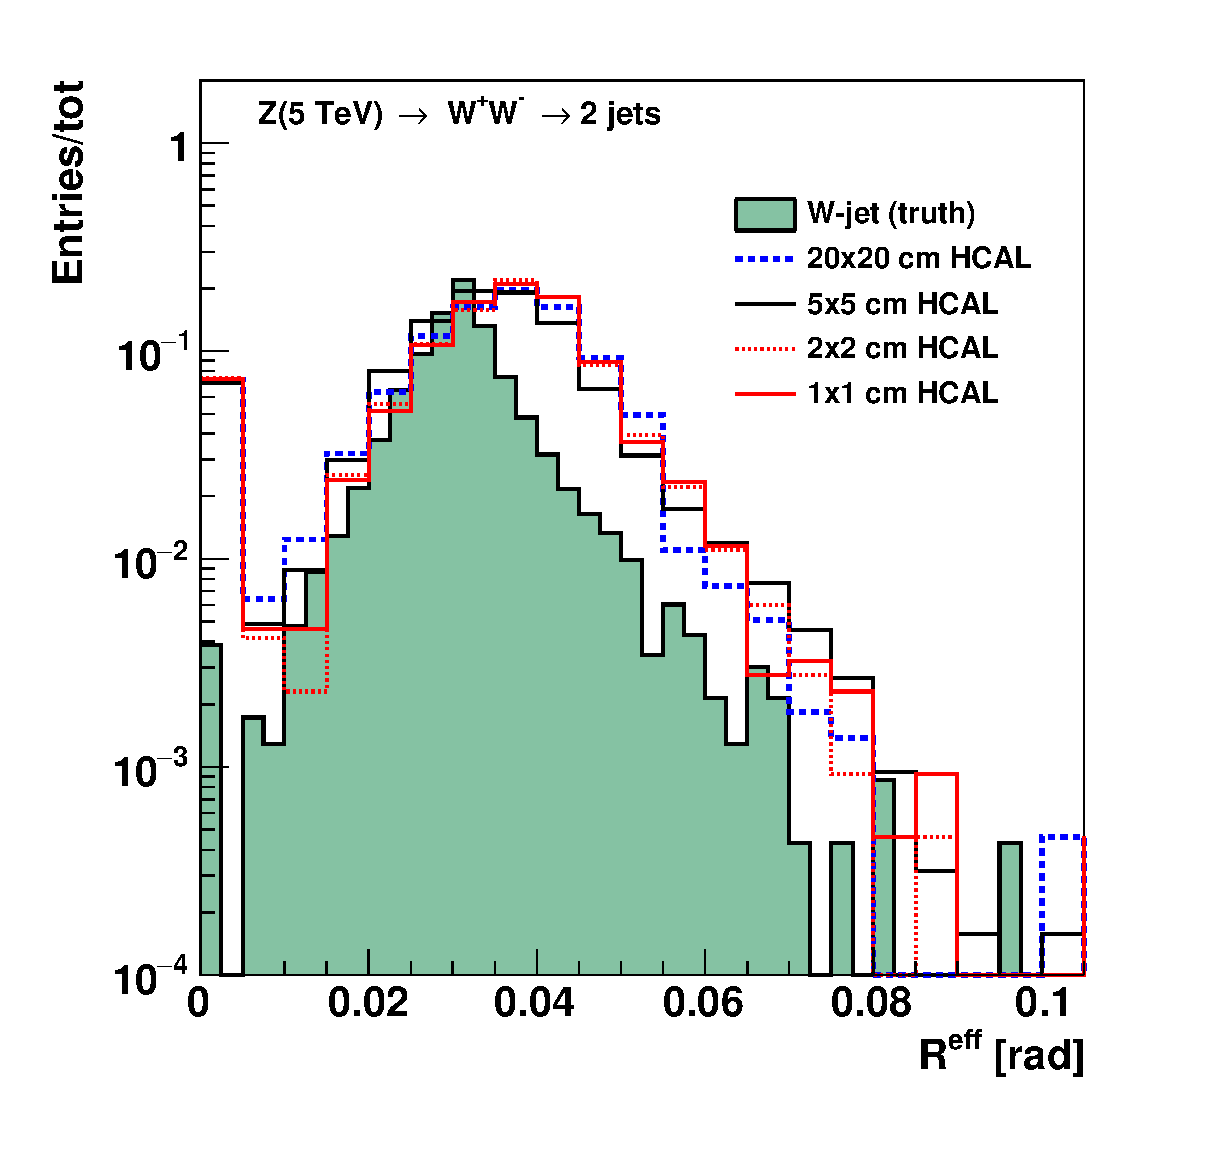
\includegraphics[width=0.43\textwidth]{figs/h5tev_clus_effR_ww1}\hfill
   }
   \subfigure[10 TeV] {
   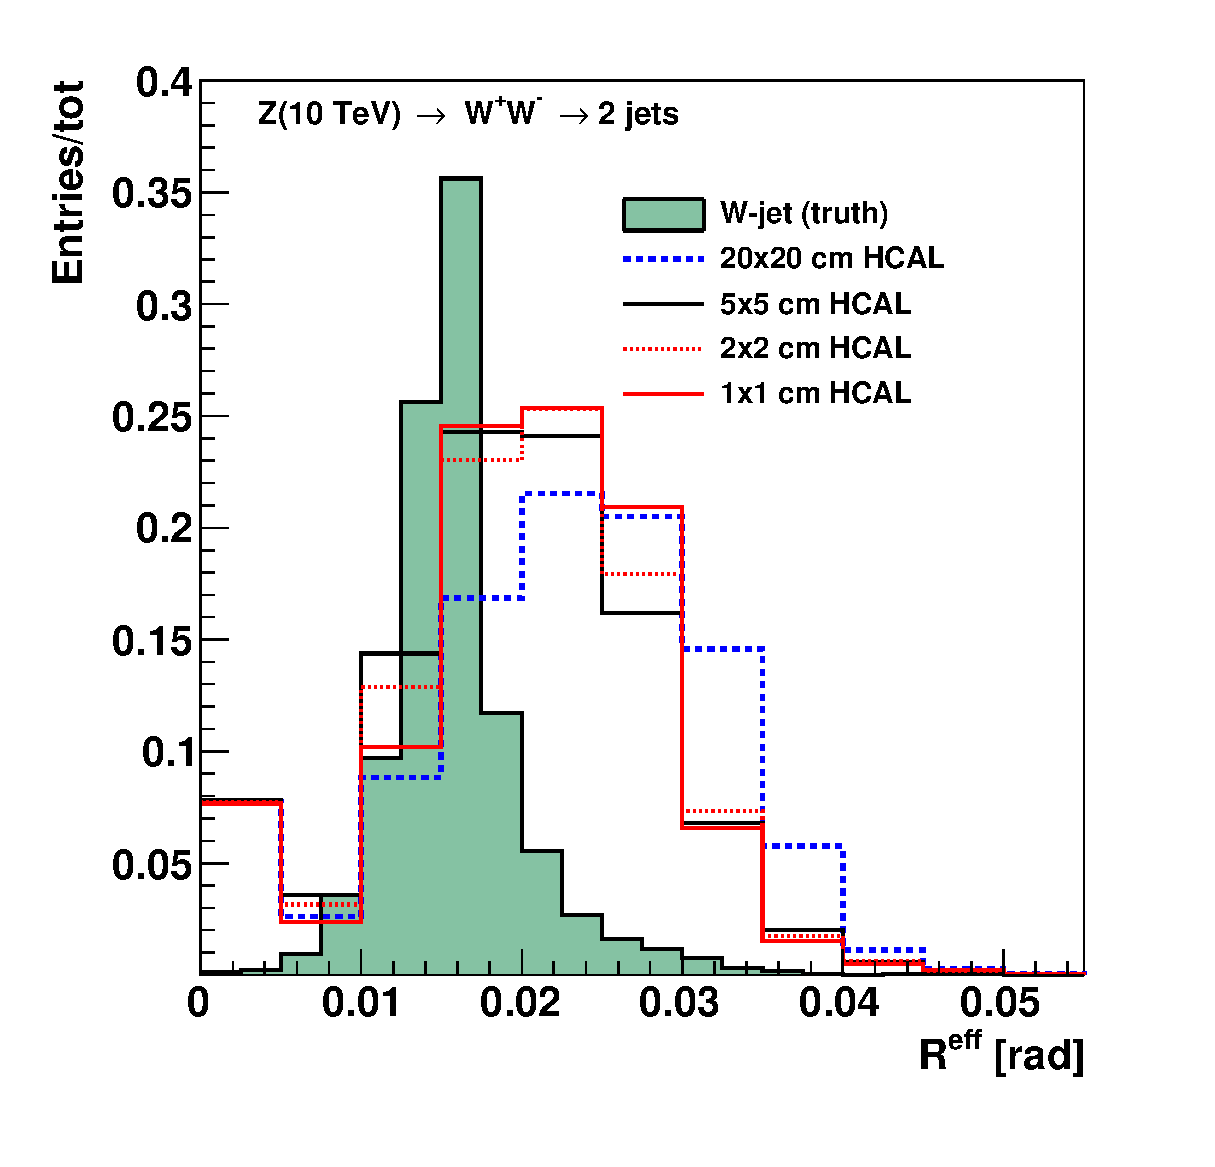
\includegraphics[width=0.43\textwidth]{figs/h10tev_clus_effR_ww1}
   }
   \subfigure[20 TeV] {
   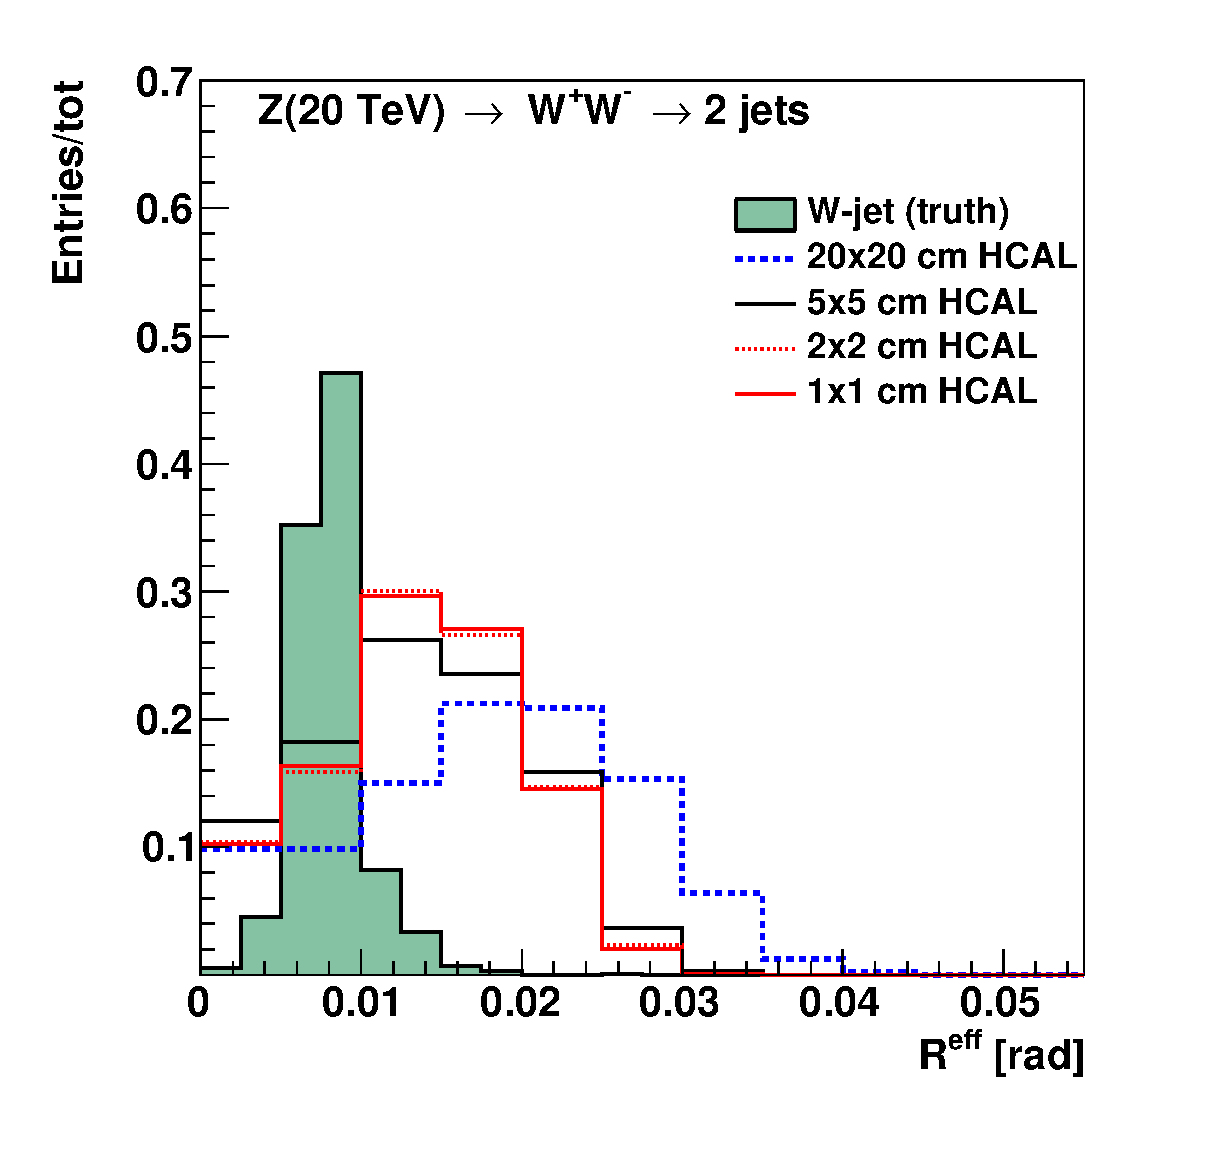
\includegraphics[width=0.43\textwidth]{figs/h20tev_clus_effR_ww1}
   }
   \subfigure[40 TeV] {
   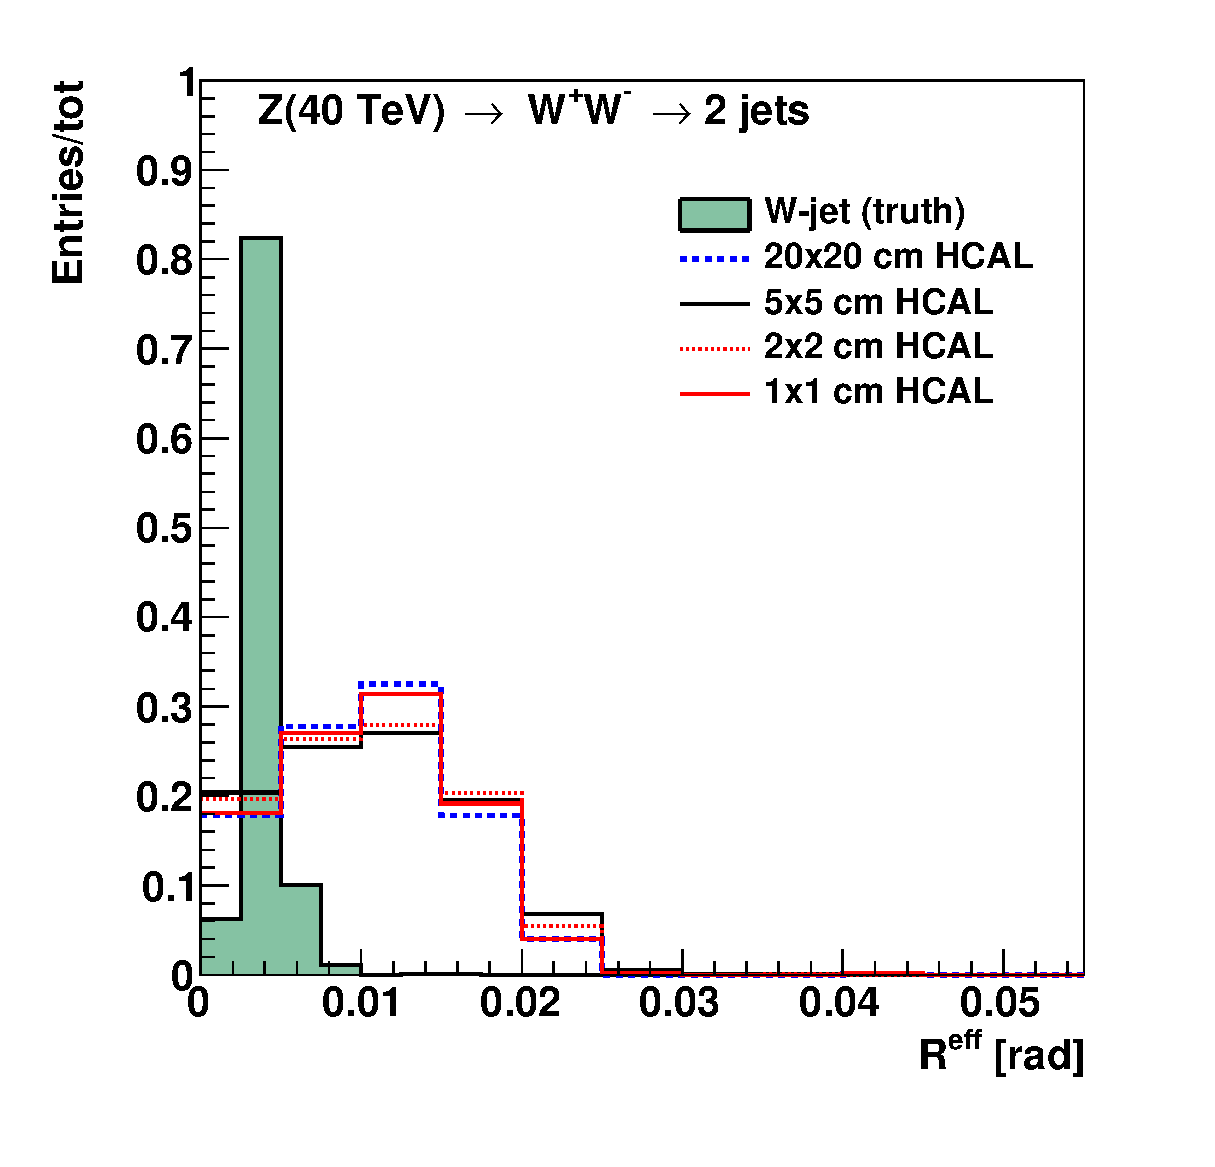
\includegraphics[width=0.43\textwidth]{figs/h40tev_clus_effR_ww1}
   }
\end{center}
\caption{Jet effective radius for different jet transverse momenta and HCAL granularities.}
\label{fig:eff_rad}
\end{figure}


Let us study the effect of granularity on jet splitting scales.
A jet $k_T$ splitting scale \cite{Butterworth:2002tt} is defined as a distance measure
used to form jets by the $k_T$ recombination
algorithm \cite{Catani1993187,Ellis:1993tq}.
This has been studied by ATLAS~\cite{ATLAS:2012am}, and more recently in the context of 100 TeV physics \cite{Auerbach:2014xua}.
The distribution of the splitting scale $\sqrt{d_{12}}=\min(p_T^1,p_T^2) \times \delta R_{12}$ \cite{ATLAS:2012am} at the final stage of the $k_T$ clustering, where two subjets are merged into the final one,
is shown in Fig.~\ref{fig:d12}.

\begin{figure}
\begin{center}
   \subfigure[5 TeV] {
   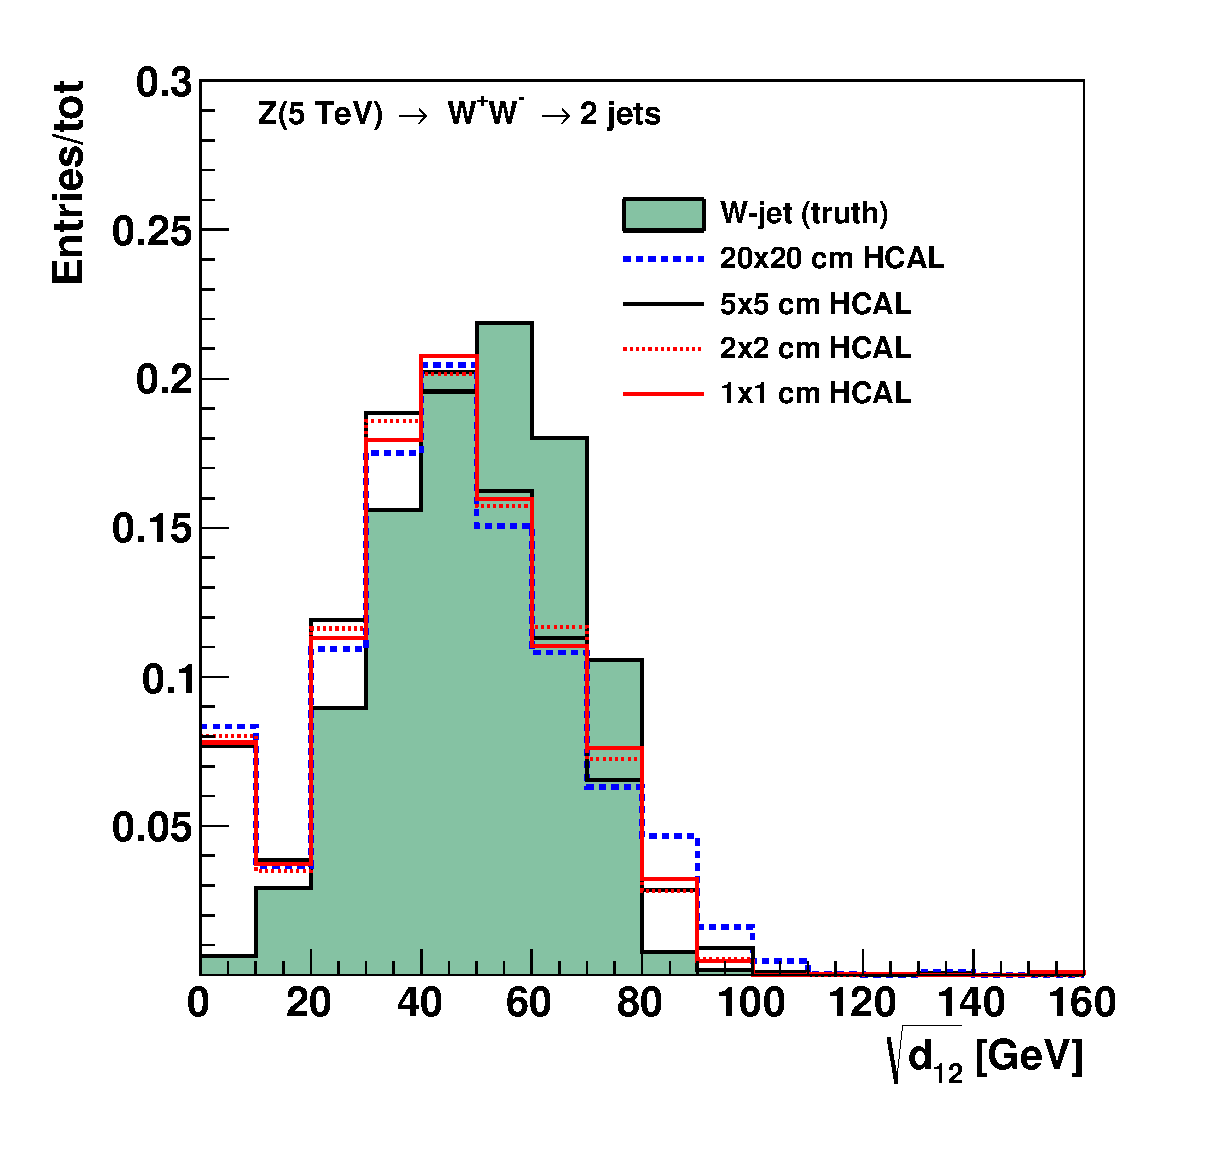
\includegraphics[width=0.43\textwidth]{figs/h5tev_clus_d12_ww1}\hfill
   }
   \subfigure[10 TeV] {
   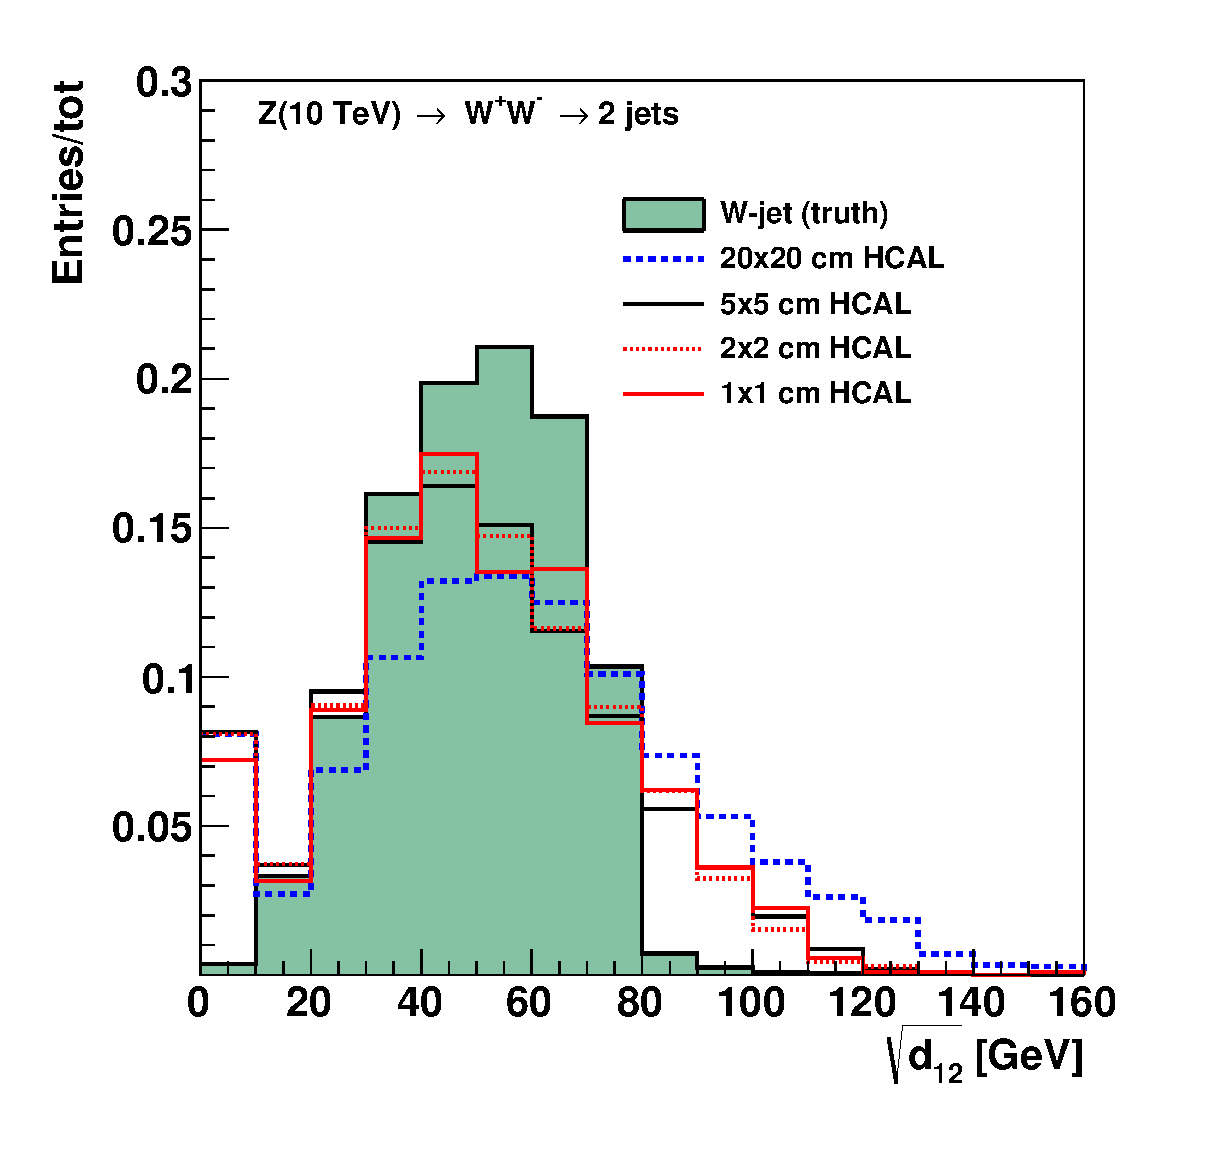
\includegraphics[width=0.43\textwidth]{figs/h10tev_clus_d12_ww1}
   }
   \subfigure[20 TeV] {
   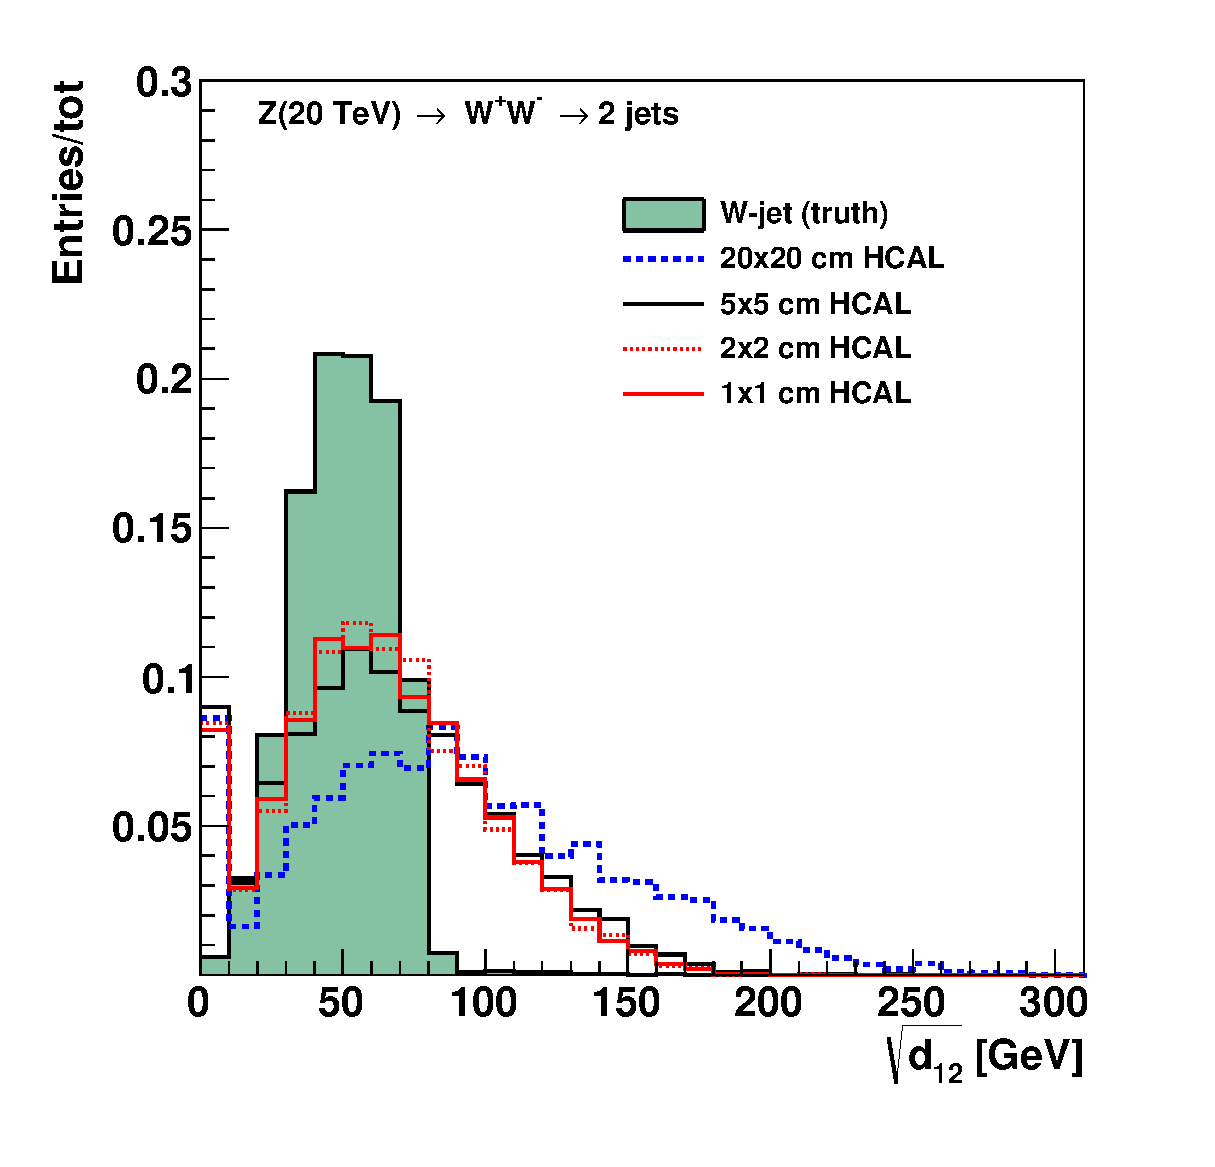
\includegraphics[width=0.43\textwidth]{figs/h20tev_clus_d12_ww1}
   }
   \subfigure[40 TeV] {
   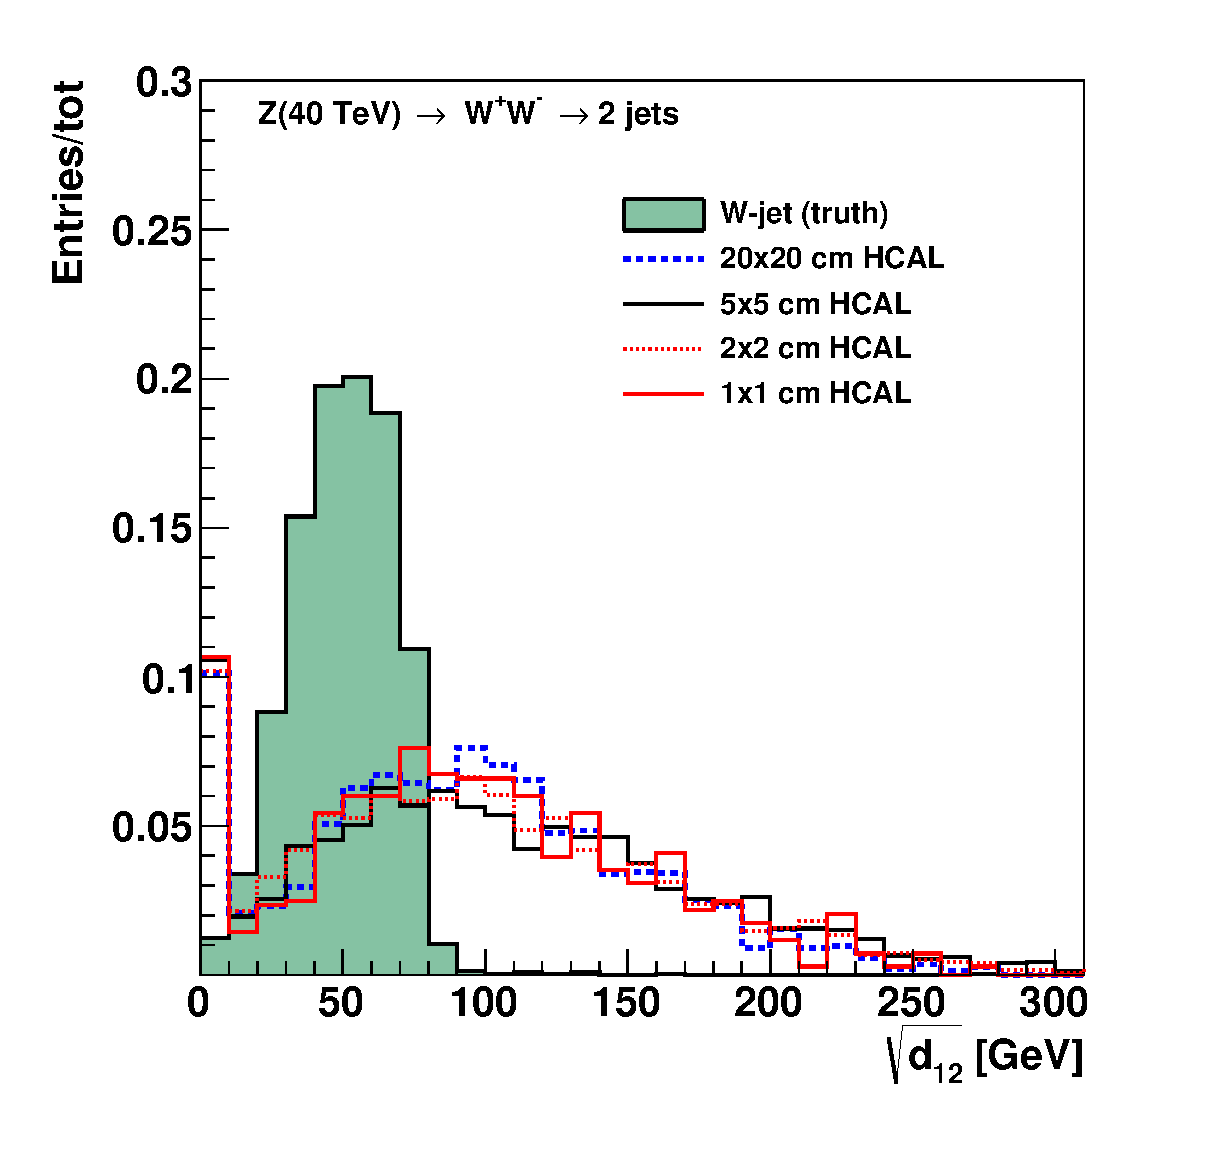
\includegraphics[width=0.43\textwidth]{figs/h40tev_clus_d12_ww1}
   }
\end{center}
\caption{Jet splitting scale for different jet transverse momenta and HCAL granularity.}
\label{fig:d12}
\end{figure}


\subsection{Jet subjettiness}

We recall that $N$-subjettiness~\cite{Thaler:2010tr}, $\tau_{N}$, of jets has been proposed
as a class of variables with which to study the decay products of a heavy particle inside jets.  $\tau_{N}$ is a measure of the degree to which a jet can be considered as being composed of
 $N$  $k_{T}$-subjets \cite{Thaler:2010tr}. 
The variable $\tau_{32}$, defined as the ratio of the $N$-subjettiness variables $\tau_3/\tau_2$, is particularly sensitive to hadronically-decaying
 top-quark initiated jets.
The variable, $\tau_{21} \equiv \tau_2/\tau_1$ can be used to reject background from $W/Z$ decays.
These variables do not strongly correlate with jet mass and can provide an independent check for the
presence of top quarks.
The jet substructure variables were obtained by re-running the $k_T$ algorithm over the jet constituents of anti-$k_T$ jets.

%%%%%%%%%%%%%%% commented out 
\begin{comment}


As an example of the effect of the calorimeter granularity, 
\begin{figure}
\begin{center}
   \subfigure[5 TeV] {
   \includegraphics[width=0.43\textwidth]{figs/r09_tau21b1_20tev_04_U.pdf}\hfill
   }
   \subfigure[10 TeV] {
   \includegraphics[width=0.43\textwidth]{figs/r010_tau21b1_20tev_04_U.pdf}
   }
   \subfigure[20 TeV] {
   \includegraphics[width=0.43\textwidth]{figs/r012_tau21b1_20tev_04_U.pdf}
   }
\end{center}
\caption{Jet subjetinness $\tau_{21}$ for jets originating from splitting scale for different jet transverse moment and HCAL granularity.}
\label{fig:tau21}
\end{figure}


\begin{figure}
\begin{center}
   \subfigure[5 TeV] {
   \includegraphics[width=0.43\textwidth]{figs/r09_tau32b1_20tev_04_U.pdf}\hfill
   }
   \subfigure[10 TeV] {
   \includegraphics[width=0.43\textwidth]{figs/r010_tau32b1_20tev_04_U.pdf}
   }
   \subfigure[20 TeV] {
   \includegraphics[width=0.43\textwidth]{figs/r012_tau32b1_20tev_04_U.pdf}
   }
\end{center}
\caption{Jet subjetinness $\tau_{32}$ for jets originating from splitting scale for different jet transverse moment and HCAL granularity.}
\label{fig:tau21}
\end{figure}

%%%%%%%%%%%%%%% commented out 
\end{comment}

